\input{header.tex}
\input{newcommands.tex}


\title{Sudokus mit dem Paket \texttt{sudoku} setzen}
\author{Fortbildungsmaterial für MINT-Lehrkräfte}
\date{\today}
\pagestyle{plain}
\setlength{\parskip}{1.5em} % Abstand zwischen Absätzen (Handreichungen)
\setlength{\emergencystretch}{2em} % lange \texttt-Wörter umbrechen statt über den Rand

% Erzeugt mit sudoku_generator.py (Stufe mittel, Seed 7)
% Sudoku A: 31 Vorgaben
\newcommand\SudokuAufgabeA{%
\begin{sudoku}
|2| | |3|6| |1|9| |.
|3| | | |9| | | | |.
| |8|1| | | |3| |7|.
| | |2|8| | | | | |.
|7| | |9|3|6| | |2|.
| | | | | |1|8| | |.
|4| |5| | | |2|8| |.
| | | | |5| | | |6|.
| |3|9| |8|2| | |5|.
\end{sudoku}}
\newcommand\SudokuLoesungA{%
\begin{sudoku}
|{\textbf{2}}|{\textcolor{black!45}{5}}|{\textcolor{black!45}{4}}|{\textbf{3}}|{\textbf{6}}|{\textcolor{black!45}{7}}|{\textbf{1}}|{\textbf{9}}|{\textcolor{black!45}{8}}|.
|{\textbf{3}}|{\textcolor{black!45}{7}}|{\textcolor{black!45}{6}}|{\textcolor{black!45}{1}}|{\textbf{9}}|{\textcolor{black!45}{8}}|{\textcolor{black!45}{5}}|{\textcolor{black!45}{2}}|{\textcolor{black!45}{4}}|.
|{\textcolor{black!45}{9}}|{\textbf{8}}|{\textbf{1}}|{\textcolor{black!45}{2}}|{\textcolor{black!45}{4}}|{\textcolor{black!45}{5}}|{\textbf{3}}|{\textcolor{black!45}{6}}|{\textbf{7}}|.
|{\textcolor{black!45}{5}}|{\textcolor{black!45}{9}}|{\textbf{2}}|{\textbf{8}}|{\textcolor{black!45}{7}}|{\textcolor{black!45}{4}}|{\textcolor{black!45}{6}}|{\textcolor{black!45}{3}}|{\textcolor{black!45}{1}}|.
|{\textbf{7}}|{\textcolor{black!45}{1}}|{\textcolor{black!45}{8}}|{\textbf{9}}|{\textbf{3}}|{\textbf{6}}|{\textcolor{black!45}{4}}|{\textcolor{black!45}{5}}|{\textbf{2}}|.
|{\textcolor{black!45}{6}}|{\textcolor{black!45}{4}}|{\textcolor{black!45}{3}}|{\textcolor{black!45}{5}}|{\textcolor{black!45}{2}}|{\textbf{1}}|{\textbf{8}}|{\textcolor{black!45}{7}}|{\textcolor{black!45}{9}}|.
|{\textbf{4}}|{\textcolor{black!45}{6}}|{\textbf{5}}|{\textcolor{black!45}{7}}|{\textcolor{black!45}{1}}|{\textcolor{black!45}{9}}|{\textbf{2}}|{\textbf{8}}|{\textcolor{black!45}{3}}|.
|{\textcolor{black!45}{8}}|{\textcolor{black!45}{2}}|{\textcolor{black!45}{7}}|{\textcolor{black!45}{4}}|{\textbf{5}}|{\textcolor{black!45}{3}}|{\textcolor{black!45}{9}}|{\textcolor{black!45}{1}}|{\textbf{6}}|.
|{\textcolor{black!45}{1}}|{\textbf{3}}|{\textbf{9}}|{\textcolor{black!45}{6}}|{\textbf{8}}|{\textbf{2}}|{\textcolor{black!45}{7}}|{\textcolor{black!45}{4}}|{\textbf{5}}|.
\end{sudoku}}

% Sudoku B: 31 Vorgaben
\newcommand\SudokuAufgabeB{%
\begin{sudoku}
|1| | | | |4| |9| |.
|4| | | | |8|5| | |.
| | | | | |9| |6| |.
|6| |1|3|4|7|8| | |.
| | |8| |9| |1| | |.
| | |3|8|6|1|7| |4|.
| |7| |2| | | | | |.
| | |4|9| | | | |5|.
| |2| |4| | | | |7|.
\end{sudoku}}
\newcommand\SudokuLoesungB{%
\begin{sudoku}
|{\textbf{1}}|{\textcolor{black!45}{6}}|{\textcolor{black!45}{2}}|{\textcolor{black!45}{7}}|{\textcolor{black!45}{5}}|{\textbf{4}}|{\textcolor{black!45}{3}}|{\textbf{9}}|{\textcolor{black!45}{8}}|.
|{\textbf{4}}|{\textcolor{black!45}{3}}|{\textcolor{black!45}{9}}|{\textcolor{black!45}{6}}|{\textcolor{black!45}{2}}|{\textbf{8}}|{\textbf{5}}|{\textcolor{black!45}{7}}|{\textcolor{black!45}{1}}|.
|{\textcolor{black!45}{5}}|{\textcolor{black!45}{8}}|{\textcolor{black!45}{7}}|{\textcolor{black!45}{1}}|{\textcolor{black!45}{3}}|{\textbf{9}}|{\textcolor{black!45}{4}}|{\textbf{6}}|{\textcolor{black!45}{2}}|.
|{\textbf{6}}|{\textcolor{black!45}{5}}|{\textbf{1}}|{\textbf{3}}|{\textbf{4}}|{\textbf{7}}|{\textbf{8}}|{\textcolor{black!45}{2}}|{\textcolor{black!45}{9}}|.
|{\textcolor{black!45}{7}}|{\textcolor{black!45}{4}}|{\textbf{8}}|{\textcolor{black!45}{5}}|{\textbf{9}}|{\textcolor{black!45}{2}}|{\textbf{1}}|{\textcolor{black!45}{3}}|{\textcolor{black!45}{6}}|.
|{\textcolor{black!45}{2}}|{\textcolor{black!45}{9}}|{\textbf{3}}|{\textbf{8}}|{\textbf{6}}|{\textbf{1}}|{\textbf{7}}|{\textcolor{black!45}{5}}|{\textbf{4}}|.
|{\textcolor{black!45}{8}}|{\textbf{7}}|{\textcolor{black!45}{6}}|{\textbf{2}}|{\textcolor{black!45}{1}}|{\textcolor{black!45}{5}}|{\textcolor{black!45}{9}}|{\textcolor{black!45}{4}}|{\textcolor{black!45}{3}}|.
|{\textcolor{black!45}{3}}|{\textcolor{black!45}{1}}|{\textbf{4}}|{\textbf{9}}|{\textcolor{black!45}{7}}|{\textcolor{black!45}{6}}|{\textcolor{black!45}{2}}|{\textcolor{black!45}{8}}|{\textbf{5}}|.
|{\textcolor{black!45}{9}}|{\textbf{2}}|{\textcolor{black!45}{5}}|{\textbf{4}}|{\textcolor{black!45}{8}}|{\textcolor{black!45}{3}}|{\textcolor{black!45}{6}}|{\textcolor{black!45}{1}}|{\textbf{7}}|.
\end{sudoku}}

 % mit sudoku_generator.py erzeugt (Stufe mittel, Seed 7)


\begin{document}

\maketitle

Sudokus sind beliebt für Vertretungsstunden, als Knobelaufgabe zum Stundenende oder als Einstieg in das Backtracking im Informatikunterricht. Mit dem Paket \texttt{sudoku} setzt \hologo{LaTeX} die Gitter sauber und einheitlich. Schwierig ist etwas anderes: Ein selbst ausgedachtes Sudoku hat fast nie genau eine Lösung. Diese Handreichung zeigt deshalb zuerst, wie man Gitter setzt und gestaltet, und dann, wie ein Python-Skript neue Rätsel samt Lösung erzeugt und vorhandene Rätsel prüft.



%%%%  KAPITEL 1  %%%%
\section{Grundlagen und benötigte Pakete}

In der universalen \texttt{header.tex} ist das Paket bereits geladen. In einem eigenständigen Dokument genügt:

\begin{lstlisting}[style=latex]
\usepackage{sudoku}
\end{lstlisting}

Das Paket \texttt{sudoku} darf nicht zusammen mit \texttt{printsudoku} oder \texttt{sudokubundle} geladen werden. Beide definieren ebenfalls einen Befehl \texttt{\textbackslash sudoku}, und die Fehlermeldung ist dann kaum zu verstehen.


%%%%  UNTERKAPITEL 1.1  %%%%
\subsection{Ein erstes Gitter}

Ein Sudoku steht in der Umgebung \texttt{sudoku}. Jede der neun Zeilen beginnt mit einem senkrechten Strich, die Zellen werden durch \texttt{|} getrennt, und am Ende jeder Zeile steht ein Punkt. Eine leere Zelle ist ein Leerzeichen.

\begin{lstlisting}[style=latex]
\begin{sudoku}
|5|3| | |7| | | | |.
|6| | |1|9|5| | | |.
| |9|8| | | | |6| |.
|8| | | |6| | | |3|.
|4| | |8| |3| | |1|.
|7| | | |2| | | |6|.
| |6| | | | |2|8| |.
| | | |4|1|9| | |5|.
| | | | |8| | |7|9|.
\end{sudoku}
\end{lstlisting}

\begin{ausgabe}
\setlength\sudokusize{8cm}
\begin{sudoku}
|5|3| | |7| | | | |.
|6| | |1|9|5| | | |.
| |9|8| | | | |6| |.
|8| | | |6| | | |3|.
|4| | |8| |3| | |1|.
|7| | | |2| | | |6|.
| |6| | | | |2|8| |.
| | | |4|1|9| | |5|.
| | | | |8| | |7|9|.
\end{sudoku}
\end{ausgabe}

Ohne weitere Angabe ist das Gitter 10\,cm breit und die Ziffern stehen in der Schriftgröße \texttt{\textbackslash Huge}; in der Ausgabe oben ist das Gitter auf 8\,cm verkleinert (siehe nächstes Kapitel). Für kleinere Gitter sollte man auch die Schrift verkleinern. Fehlt am Zeilenende der Punkt, verrutscht das ganze Gitter. Deshalb darf auch in einer Zelle kein Punkt stehen.



%%%%  KAPITEL 2  %%%%
\section{Größe, Linien und Schrift}

Das Aussehen wird über drei Längen und einen Befehl gesteuert: \texttt{\textbackslash sudokusize} ist die Kantenlänge, \texttt{\textbackslash sudokuthinline} und \texttt{\textbackslash sudokuthickline} sind die Strichstärken innerhalb und zwischen den $3\times3$-Blöcken, \texttt{\textbackslash sudokuformat} legt die Schrift jeder Zelle fest.

\begin{lstlisting}[style=latex]
\setlength\sudokusize{6cm}
\setlength\sudokuthinline{0.4pt}
\setlength\sudokuthickline{1.6pt}
\renewcommand*\sudokuformat[1]{\Large\sffamily#1}
\begin{sudoku}
|5|3| | |7| | | | |.
|6| | |1|9|5| | | |.
| |9|8| | | | |6| |.
|8| | | |6| | | |3|.
|4| | |8| |3| | |1|.
|7| | | |2| | | |6|.
| |6| | | | |2|8| |.
| | | |4|1|9| | |5|.
| | | | |8| | |7|9|.
\end{sudoku}
\end{lstlisting}

\begin{ausgabe}
\setlength\sudokusize{6cm}
\setlength\sudokuthinline{0.4pt}
\setlength\sudokuthickline{1.6pt}
\renewcommand*\sudokuformat[1]{\Large\sffamily#1}
\begin{sudoku}
|5|3| | |7| | | | |.
|6| | |1|9|5| | | |.
| |9|8| | | | |6| |.
|8| | | |6| | | |3|.
|4| | |8| |3| | |1|.
|7| | | |2| | | |6|.
| |6| | | | |2|8| |.
| | | |4|1|9| | |5|.
| | | | |8| | |7|9|.
\end{sudoku}
\end{ausgabe}

Die Einstellungen gelten bis zum Ende der aktuellen Gruppe. Stehen sie in der Präambel, gelten sie für alle Sudokus des Dokuments, so sehen alle Rätsel eines Arbeitsblatts gleich aus.



%%%%  KAPITEL 3  %%%%
\section{Zellen hervorheben}

In eine Zelle darf auch ein Befehl geschrieben werden, etwa für Fettdruck oder Farbe. Dann muss der Inhalt der Zelle in geschweiften Klammern stehen: \texttt{|\{\textbackslash textbf\{5\}\}|}. Ohne Klammern liest das Trennzeichen \texttt{|} nur das erste Zeichen, und \hologo{LaTeX} bricht mit \enquote{Argument of \textbackslash textcolor has an extra \}} ab.

Das Beispiel zeigt eine Lösung, in der die Vorgaben fett und die ergänzten Ziffern grau gesetzt sind. Die mittlere Zeile ist zusätzlich rot markiert:

\begin{lstlisting}[style=latex]
\setlength\sudokusize{6cm}
\renewcommand*\sudokuformat[1]{\Large\sffamily#1}
\newcommand\vor[1]{{\textbf{#1}}}
\newcommand\erg[1]{{\textcolor{black!45}{#1}}}
\newcommand\rot[1]{{\textcolor{red}{\textbf{#1}}}}
\begin{sudoku}
|{\vor5}|{\vor3}|{\erg4}|{\erg6}|{\vor7}|{\erg8}|{\erg9}|{\erg1}|{\erg2}|.
|{\vor6}|{\erg7}|{\erg2}|{\vor1}|{\vor9}|{\vor5}|{\erg3}|{\erg4}|{\erg8}|.
|{\erg1}|{\vor9}|{\vor8}|{\erg3}|{\erg4}|{\erg2}|{\erg5}|{\vor6}|{\erg7}|.
|{\vor8}|{\erg5}|{\erg9}|{\erg7}|{\vor6}|{\erg1}|{\erg4}|{\erg2}|{\vor3}|.
|{\rot4}|{\rot2}|{\rot6}|{\rot8}|{\rot5}|{\rot3}|{\rot7}|{\rot9}|{\rot1}|.
|{\vor7}|{\erg1}|{\erg3}|{\erg9}|{\vor2}|{\erg4}|{\erg8}|{\erg5}|{\vor6}|.
|{\erg9}|{\vor6}|{\erg1}|{\erg5}|{\erg3}|{\erg7}|{\vor2}|{\vor8}|{\erg4}|.
|{\erg2}|{\erg8}|{\erg7}|{\vor4}|{\vor1}|{\vor9}|{\erg6}|{\erg3}|{\vor5}|.
|{\erg3}|{\erg4}|{\erg5}|{\erg2}|{\vor8}|{\erg6}|{\erg1}|{\vor7}|{\vor9}|.
\end{sudoku}
\end{lstlisting}

\begin{ausgabe}
\setlength\sudokusize{6cm}
\renewcommand*\sudokuformat[1]{\Large\sffamily#1}
\newcommand\vor[1]{{\textbf{#1}}}
\newcommand\erg[1]{{\textcolor{black!45}{#1}}}
\newcommand\rot[1]{{\textcolor{red}{\textbf{#1}}}}
\begin{sudoku}
|{\vor5}|{\vor3}|{\erg4}|{\erg6}|{\vor7}|{\erg8}|{\erg9}|{\erg1}|{\erg2}|.
|{\vor6}|{\erg7}|{\erg2}|{\vor1}|{\vor9}|{\vor5}|{\erg3}|{\erg4}|{\erg8}|.
|{\erg1}|{\vor9}|{\vor8}|{\erg3}|{\erg4}|{\erg2}|{\erg5}|{\vor6}|{\erg7}|.
|{\vor8}|{\erg5}|{\erg9}|{\erg7}|{\vor6}|{\erg1}|{\erg4}|{\erg2}|{\vor3}|.
|{\rot4}|{\rot2}|{\rot6}|{\rot8}|{\rot5}|{\rot3}|{\rot7}|{\rot9}|{\rot1}|.
|{\vor7}|{\erg1}|{\erg3}|{\erg9}|{\vor2}|{\erg4}|{\erg8}|{\erg5}|{\vor6}|.
|{\erg9}|{\vor6}|{\erg1}|{\erg5}|{\erg3}|{\erg7}|{\vor2}|{\vor8}|{\erg4}|.
|{\erg2}|{\erg8}|{\erg7}|{\vor4}|{\vor1}|{\vor9}|{\erg6}|{\erg3}|{\vor5}|.
|{\erg3}|{\erg4}|{\erg5}|{\erg2}|{\vor8}|{\erg6}|{\erg1}|{\vor7}|{\vor9}|.
\end{sudoku}
\end{ausgabe}

Die Hilfsbefehle \texttt{\textbackslash vor}, \texttt{\textbackslash erg} und \texttt{\textbackslash rot} halten das Gitter kurz. Auch sie müssen in der Zelle in Klammern stehen: \texttt{|\{\textbackslash vor5\}|}.



%%%%  KAPITEL 4  %%%%
\section{Neue Rätsel erzeugen}


%%%%  UNTERKAPITEL 4.1  %%%%
\subsection{Der Generator}

Neue Sudokus erzeugt das Python-Skript \texttt{sudoku\_generator.py} aus dem Ordner \texttt{scripts} des Skills. Es füllt zuerst ein vollständiges Gitter und streicht dann so lange Ziffern, bis die gewünschte Schwierigkeit erreicht ist. Nach jedem Streichen prüft es per Backtracking, ob es noch genau eine Lösung gibt. Der Aufruf im Terminal:

\begin{lstlisting}[style=latex]
python3 sudoku_generator.py -n 2 -s mittel --seed 7 -o beispiel_sudokus.tex
\end{lstlisting}

\begin{itemize}
	\item \texttt{-n 2} erzeugt zwei Rätsel.
	\item \texttt{-s leicht}, \texttt{mittel} oder \texttt{schwer} legt die Zahl der Vorgaben fest (etwa 40, 32 oder 26).
	\item \texttt{-{}-seed 7} macht das Ergebnis wiederholbar: Mit derselben Zahl entstehen dieselben Rätsel. Für Parallelklassen nimmt man verschiedene Zahlen.
	\item \texttt{-o} gibt die Zieldatei an.
\end{itemize}


%%%%  UNTERKAPITEL 4.2  %%%%
\subsection{Die erzeugten Rätsel einbinden}

Die erzeugte Datei enthält für jedes Rätsel zwei Befehle: \texttt{\textbackslash SudokuAufgabeA} und \texttt{\textbackslash SudokuLoesungA}, dann \texttt{\textbackslash SudokuAufgabeB} und so weiter. Man lädt sie in der Präambel:

\begin{lstlisting}[style=latex]
% Erzeugt mit sudoku_generator.py (Stufe mittel, Seed 7)
% Sudoku A: 31 Vorgaben
\newcommand\SudokuAufgabeA{%
\begin{sudoku}
|2| | |3|6| |1|9| |.
|3| | | |9| | | | |.
| |8|1| | | |3| |7|.
| | |2|8| | | | | |.
|7| | |9|3|6| | |2|.
| | | | | |1|8| | |.
|4| |5| | | |2|8| |.
| | | | |5| | | |6|.
| |3|9| |8|2| | |5|.
\end{sudoku}}
\newcommand\SudokuLoesungA{%
\begin{sudoku}
|{\textbf{2}}|{\textcolor{black!45}{5}}|{\textcolor{black!45}{4}}|{\textbf{3}}|{\textbf{6}}|{\textcolor{black!45}{7}}|{\textbf{1}}|{\textbf{9}}|{\textcolor{black!45}{8}}|.
|{\textbf{3}}|{\textcolor{black!45}{7}}|{\textcolor{black!45}{6}}|{\textcolor{black!45}{1}}|{\textbf{9}}|{\textcolor{black!45}{8}}|{\textcolor{black!45}{5}}|{\textcolor{black!45}{2}}|{\textcolor{black!45}{4}}|.
|{\textcolor{black!45}{9}}|{\textbf{8}}|{\textbf{1}}|{\textcolor{black!45}{2}}|{\textcolor{black!45}{4}}|{\textcolor{black!45}{5}}|{\textbf{3}}|{\textcolor{black!45}{6}}|{\textbf{7}}|.
|{\textcolor{black!45}{5}}|{\textcolor{black!45}{9}}|{\textbf{2}}|{\textbf{8}}|{\textcolor{black!45}{7}}|{\textcolor{black!45}{4}}|{\textcolor{black!45}{6}}|{\textcolor{black!45}{3}}|{\textcolor{black!45}{1}}|.
|{\textbf{7}}|{\textcolor{black!45}{1}}|{\textcolor{black!45}{8}}|{\textbf{9}}|{\textbf{3}}|{\textbf{6}}|{\textcolor{black!45}{4}}|{\textcolor{black!45}{5}}|{\textbf{2}}|.
|{\textcolor{black!45}{6}}|{\textcolor{black!45}{4}}|{\textcolor{black!45}{3}}|{\textcolor{black!45}{5}}|{\textcolor{black!45}{2}}|{\textbf{1}}|{\textbf{8}}|{\textcolor{black!45}{7}}|{\textcolor{black!45}{9}}|.
|{\textbf{4}}|{\textcolor{black!45}{6}}|{\textbf{5}}|{\textcolor{black!45}{7}}|{\textcolor{black!45}{1}}|{\textcolor{black!45}{9}}|{\textbf{2}}|{\textbf{8}}|{\textcolor{black!45}{3}}|.
|{\textcolor{black!45}{8}}|{\textcolor{black!45}{2}}|{\textcolor{black!45}{7}}|{\textcolor{black!45}{4}}|{\textbf{5}}|{\textcolor{black!45}{3}}|{\textcolor{black!45}{9}}|{\textcolor{black!45}{1}}|{\textbf{6}}|.
|{\textcolor{black!45}{1}}|{\textbf{3}}|{\textbf{9}}|{\textcolor{black!45}{6}}|{\textbf{8}}|{\textbf{2}}|{\textcolor{black!45}{7}}|{\textcolor{black!45}{4}}|{\textbf{5}}|.
\end{sudoku}}

% Sudoku B: 31 Vorgaben
\newcommand\SudokuAufgabeB{%
\begin{sudoku}
|1| | | | |4| |9| |.
|4| | | | |8|5| | |.
| | | | | |9| |6| |.
|6| |1|3|4|7|8| | |.
| | |8| |9| |1| | |.
| | |3|8|6|1|7| |4|.
| |7| |2| | | | | |.
| | |4|9| | | | |5|.
| |2| |4| | | | |7|.
\end{sudoku}}
\newcommand\SudokuLoesungB{%
\begin{sudoku}
|{\textbf{1}}|{\textcolor{black!45}{6}}|{\textcolor{black!45}{2}}|{\textcolor{black!45}{7}}|{\textcolor{black!45}{5}}|{\textbf{4}}|{\textcolor{black!45}{3}}|{\textbf{9}}|{\textcolor{black!45}{8}}|.
|{\textbf{4}}|{\textcolor{black!45}{3}}|{\textcolor{black!45}{9}}|{\textcolor{black!45}{6}}|{\textcolor{black!45}{2}}|{\textbf{8}}|{\textbf{5}}|{\textcolor{black!45}{7}}|{\textcolor{black!45}{1}}|.
|{\textcolor{black!45}{5}}|{\textcolor{black!45}{8}}|{\textcolor{black!45}{7}}|{\textcolor{black!45}{1}}|{\textcolor{black!45}{3}}|{\textbf{9}}|{\textcolor{black!45}{4}}|{\textbf{6}}|{\textcolor{black!45}{2}}|.
|{\textbf{6}}|{\textcolor{black!45}{5}}|{\textbf{1}}|{\textbf{3}}|{\textbf{4}}|{\textbf{7}}|{\textbf{8}}|{\textcolor{black!45}{2}}|{\textcolor{black!45}{9}}|.
|{\textcolor{black!45}{7}}|{\textcolor{black!45}{4}}|{\textbf{8}}|{\textcolor{black!45}{5}}|{\textbf{9}}|{\textcolor{black!45}{2}}|{\textbf{1}}|{\textcolor{black!45}{3}}|{\textcolor{black!45}{6}}|.
|{\textcolor{black!45}{2}}|{\textcolor{black!45}{9}}|{\textbf{3}}|{\textbf{8}}|{\textbf{6}}|{\textbf{1}}|{\textbf{7}}|{\textcolor{black!45}{5}}|{\textbf{4}}|.
|{\textcolor{black!45}{8}}|{\textbf{7}}|{\textcolor{black!45}{6}}|{\textbf{2}}|{\textcolor{black!45}{1}}|{\textcolor{black!45}{5}}|{\textcolor{black!45}{9}}|{\textcolor{black!45}{4}}|{\textcolor{black!45}{3}}|.
|{\textcolor{black!45}{3}}|{\textcolor{black!45}{1}}|{\textbf{4}}|{\textbf{9}}|{\textcolor{black!45}{7}}|{\textcolor{black!45}{6}}|{\textcolor{black!45}{2}}|{\textcolor{black!45}{8}}|{\textbf{5}}|.
|{\textcolor{black!45}{9}}|{\textbf{2}}|{\textcolor{black!45}{5}}|{\textbf{4}}|{\textcolor{black!45}{8}}|{\textcolor{black!45}{3}}|{\textcolor{black!45}{6}}|{\textcolor{black!45}{1}}|{\textbf{7}}|.
\end{sudoku}}


\end{lstlisting}

 Danach lassen sich die Rätsel überall aufrufen, zum Beispiel nebeneinander in zwei \texttt{minipage}-Umgebungen:

\begin{lstlisting}[style=latex]
\setlength\sudokusize{6.5cm}
\renewcommand*\sudokuformat[1]{\Large\sffamily#1}
\begin{minipage}[t]{0.48\linewidth}\centering
	\textbf{Aufgabe}
	\SudokuAufgabeA
\end{minipage}\hfill
\begin{minipage}[t]{0.48\linewidth}\centering
	\textbf{Lösung}
	\SudokuLoesungA
\end{minipage}
\end{lstlisting}

\begin{ausgabe}
\setlength\sudokusize{6.5cm}
\renewcommand*\sudokuformat[1]{\Large\sffamily#1}
\begin{minipage}[t]{0.48\linewidth}\centering
	\textbf{Aufgabe}
	\SudokuAufgabeA
\end{minipage}\hfill
\begin{minipage}[t]{0.48\linewidth}\centering
	\textbf{Lösung}
	\SudokuLoesungA
\end{minipage}
\end{ausgabe}

In der Lösung stehen die Vorgaben fett und die ergänzten Ziffern grau, so findet man beim Kontrollieren schnell die Stelle, an der ein Fehler liegt. Im Ordner \texttt{assets} des Skills liegt ein fertiges Arbeitsblatt mit vier Rätseln auf der Vorderseite und den Lösungen auf der Rückseite. Die Datei heißt \texttt{vorlage\_sudoku\_arbeitsblatt.tex}.


%%%%  UNTERKAPITEL 4.3  %%%%
\subsection{Ein vorhandenes Sudoku prüfen}

Sudokus aus Zeitungen oder Rätselheften lassen sich mit demselben Skript lösen und prüfen. Dazu schreibt man das Gitter zeilenweise als 81 Zeichen auf, eine leere Zelle ist ein Punkt:

\begin{lstlisting}[style=latex]
python3 sudoku_generator.py --loesen "53..7....6..195....98....6.8...6...34..8.3..17...2...6.6....28....419..5....8..79"
\end{lstlisting}

Das Skript gibt den \hologo{LaTeX}-Code für Aufgabe und Lösung aus und warnt, wenn das Rätsel mehr als eine Lösung hat. Das ist bei selbst ausgedachten Sudokus fast immer der Fall.



%%%%  KAPITEL 5  %%%%
\section{Mini-Sudokus mit \TikZ}

Das Paket kennt nur das $9\times9$-Gitter. Für die Klassen 5 und 6 eignen sich kleinere Sudokus mit $4\times4$ Feldern und den Ziffern 1 bis 4. Sie lassen sich mit \TikZ zeichnen: ein dünnes Gitter, darüber dicke Linien für die $2\times2$-Blöcke, dann die Vorgaben.

\begin{lstlisting}[style=latex]
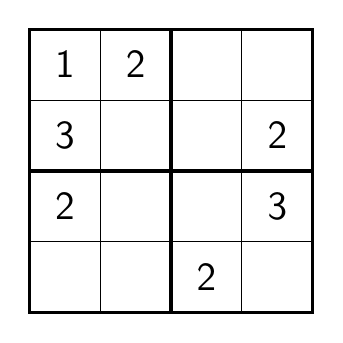
\begin{tikzpicture}[scale=0.9]
	\draw[step=1, thin] (0,0) grid (4,4);
	\draw[very thick] (0,0) rectangle (4,4) (2,0) -- (2,4) (0,2) -- (4,2);
	\foreach \x/\y/\z in {0/3/1, 1/3/2, 0/2/3, 3/2/2, 0/1/2, 3/1/3, 2/0/2}
		\node[font=\Large\sffamily] at (\x+0.5,\y+0.5) {\z};
\end{tikzpicture}
\end{lstlisting}

\begin{ausgabe}
\centering
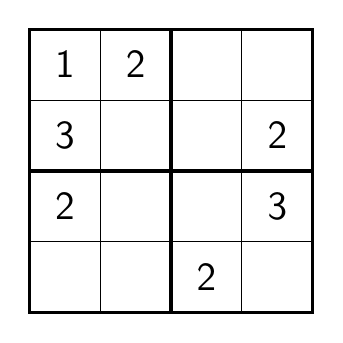
\begin{tikzpicture}[scale=0.9]
	\draw[step=1, thin] (0,0) grid (4,4);
	\draw[very thick] (0,0) rectangle (4,4) (2,0) -- (2,4) (0,2) -- (4,2);
	\foreach \x/\y/\z in {0/3/1, 1/3/2, 0/2/3, 3/2/2, 0/1/2, 3/1/3, 2/0/2}
		\node[font=\Large\sffamily] at (\x+0.5,\y+0.5) {\z};
\end{tikzpicture}
\end{ausgabe}

In der Liste stehen Spalte, Zeile (von unten gezählt) und Ziffer. Dieses Rätsel hat genau eine Lösung, das wurde durch Ausprobieren aller Möglichkeiten geprüft. Bei eigenen Mini-Sudokus muss man die Eindeutigkeit selbst prüfen, denn der Generator arbeitet nur mit $9\times9$-Gittern.



%%%%  KAPITEL 6  %%%%
\section{Zusammenfassung}

Die wichtigsten Techniken im Überblick:

\begin{itemize}
	\item Ein Gitter steht in \texttt{\textbackslash begin\{sudoku\}} \dots\ \texttt{\textbackslash end\{sudoku\}}: neun Zeilen, Zellen durch \texttt{|} getrennt, Punkt am Zeilenende.
	\item Größe, Linien und Schrift mit \texttt{\textbackslash sudokusize}, \texttt{\textbackslash sudokuthinline}, \texttt{\textbackslash sudokuthickline} und \texttt{\textbackslash sudokuformat}.
	\item Befehle in einer Zelle immer in geschweifte Klammern setzen.
	\item Rätsel nicht selbst ausdenken, sondern mit \texttt{sudoku\_generator.py} erzeugen; vorhandene Rätsel mit \texttt{-{}-loesen} prüfen.
	\item Für $4\times4$-Sudokus ein Gitter mit \TikZ zeichnen und die Eindeutigkeit selbst prüfen.
\end{itemize}

Im Informatikunterricht ist das Sudoku ein anschauliches Beispiel für Backtracking: Die Funktion \texttt{loese()} im Generator ist kurz genug, um sie gemeinsam zu lesen. Eine gute Frage dazu ist, warum es so viel schneller geht, wenn man immer zuerst das Feld mit den wenigsten möglichen Ziffern ausfüllt. In der Mathematik passt die Frage, wie viele Vorgaben ein eindeutiges Sudoku mindestens braucht. Die Antwort 17 wurde erst 2012 mit Computerhilfe bewiesen.

\end{document}
